\RequirePackage[header={{Header goes here}}]{../../latex/defaultpackage}

% glossary
\newglossaryentry{thing}
{
	name=thing,
	description={A thing.}
}
\makeglossaries

%------------------------------------

\begin{document}

%------------------------------------

\thispagestyle{empty}
\begin{center}
	
	\bigskip
	\bigskip

	\huge Title

	\bigskip
	\bigskip

	\begin{large}
		\begin{tabular}{ r l }
			\b{Student} & Mark Ormesher \\
			& 1301981 \\

			& \\

			\b{Extra Detail} & Line 1 \\
			& Line 2 \\
			& Line 3 \\

			& \\

			\b{Report Submission} & \todo{1st January 1960}
		\end{tabular}
	\end{large}

\end{center}

%------------------------------------

\clearpage
\section{Originality Avowal}

I verify that I am the sole author of this report, except where explicitly stated to the contrary.

\bigskip
\bigskip

\noindent\rule{4cm}{0.4pt}
\noindent{Mark Ormesher}

\bigskip
\bigskip

\noindent\rule{4cm}{0.4pt}
\noindent{Date}

%------------------------------------

\clearpage
\setlength{\parskip}{0em}
\tableofcontents
\setlength{\parskip}{\baselineskip}

%------------------------------------

\clearpage
\section{Section}

Section content~\cite{TemplateCitation2016}.

This \gls{thing} needs to be defined.

Figure \ref{fig:stock} in \nameref{section:portfolio} on page \pageref{section:portfolio} shows a stock photo of stock.

%------------------------------------

\clearpage
\section{Appendix A: Portfolio} \label{section:portfolio}

\begin{figure}[!htb]
	\begin{center}
		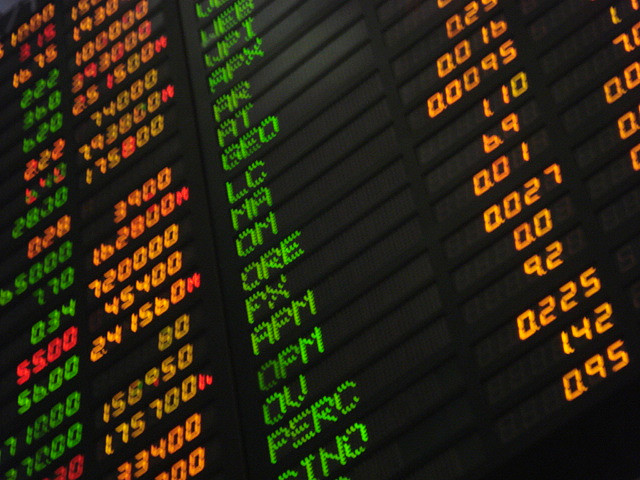
\includegraphics[width=0.5\textwidth]{stock}
		\caption{Stock photo of stock}
		\label{fig:stock}
	\end{center}
\end{figure}

%------------------------------------

\clearpage
\section{Appendix B: Glossary} \label{glossary}

\glsresetall
\printglossary

%------------------------------------

\clearpage
\section{Appendix C: Bibliography} \label{bibliography}

\begin{flushleft}
\bibliography{template}
\end{flushleft}

%------------------------------------

\end{document}}